\chapter{Pathogenic bacteria can effect the endogenous actin cytoskeleton}\label{ch:vibrio}

\section[Abstract]{Abstract\footnotemark}
\textit{Vibrio cholera} has multiple ways to interfere with a host cell’s actin cytoskeletal system. I collaborated with two projects to better understand the different pathways that pathogenic bacteria can hijack the actin cytoskeleton. More here...

The first collaboration with Tom Burke in the Kovar lab focused on the mechanism of actin nucleators VopL and VopF. These \textit{Vibrio} nucleators assemble actin into unproductive filament. There was controversy surrounding how these proteins were able to nucleate actin filaments and we presented a solution to this controversy, showing that in the presence of physiological conditions that VopL and VopF bind to the pointed ends of F-actin. With the second collaboration with the Kudryashov lab at The Ohio State University, I used single-molecule TIRF to visualize the effect of ACD toxin formed actin oligomers on Ena/VASP. The Kudryashov lab had previously found that these toxic oligomers effect formin elongation \citep{heisler_acd_2015}, and we expanded this study to other endogenous actin assembly factors. 

Overall these two works contribute to understanding the role that pathogenic bacteria can interfere with a host's actin cytoskeleton. Understanding how \textit{Vibrio} can hijack the endogenous actin system allows us to better fight the disease-causing bacteria. I have presented below the parts of the collaborations that I had a role collecting and analyzing and focus on the aspects that are relevant to my contribution. 

\footnotetext{Citations for chapter: [1] Thomas A. Burke, Alyssa J. Harker, Roberto Dominguez, and David R. Kovar. The bacterial virulence factors VopL and VopF nucleate actin from the pointed end. \textit{The Journal of Cell Biology}, March 2017. [2] Elena Kudryashova, David B. Heisler, Blake Williams, Alyssa J. Harker, Kyle Shafer, Margot E. Quinlan, David R. Kovar, Dimitrios Vavylonis, and Dmitri S. Kudryashov. Actin Cross-Linking Toxin Is a Universal Inhibitor of Tandem-Organized and Oliogmeric G-Actin Binding Proteins. \textit{Current biology}, 28{10}:1536-1547.e9, May 2018.}

\section{Introduction}\label{ch04-introduction}
Bacterial toxins can effectively compromise a host cell's functions with relatively few molecules, even leading to cell death. These toxins can target signaling cascades (ex. cGMP, adenylate cyclase) or inhibit other enzymes important for cellular processes such as protein synthesis \citep{henkel_toxins_2010}. As the actin cyctoskeleton is important for many cellular processes, it is commonly targeted by bacterial toxins. The actin cross-linking domain toxin (ACD) of \textit{Vibrio} species and related bacterial genera are deliverd to host cells by type 1 (MARTX toxin) or type VI (VgrG1 toxin) secretion systems. ACD catalyzes formation of actin oligomers through covalent crosslinking of Lys\textsuperscript{50} in subdomain 2 of an actin monomer with Glu\textsuperscript{270} in subdomain 3 of another actin monomer by an amide bond \citep{kudryashov_connecting_2008,kudryashova_glutamyl_2012}. This results in an oligomer that is not suitable for further actin polymerization because the two monomers are oriented similar to actin subunits along the short pitch of an actin filament, except that subdomain 2 has a major twist, disrupting the normal interface for further monomer binding \citep{kudryashov_connecting_2008}.  

However, there is a high concentration of actin yet only few ACD molecules secreted into the host cell. Using in vitro determined rates of ACD activity, it would take more than 6 months to covalently crosslink half of all the cytoplasmic actin with a single ACD molecule. This is beyond the timescale for in vivo measurements of monolayer disruption \citep{}. Previously, in a collaboration with the Kudryashov lab, we found that ACD is effective not by sequestering monomers as previously thought but by using actin oligomers to target formins. \citep{heisler_acd_2015}. We found that ACD formed toxic actin oligomers that blocked formin-mediated actin polymerization and nucleation. However, the mechanism of how these ACD-formed oligomers block formin activity remains unclear. 

Another way that Vibrio species target the actin cytoskeleton is through actin assembly proteins VopF or VopL. \citep{burke_bacterial_2017}

Actin nucleators: WH2 domains
	Controversy

\section{Results}\label{ch04-results}

\subsection{Ena/VASP is inhibited by actin crosslinking toxins}\label{ena-acd-oligomers}
Our previous study showed that formin mediated elongation of F-actin is blocked by the ACD oligomers. To further understand the mechanism of how these ACD oligomers affected actin nucleators we also tested Ena/VASP. We used single-molecule TIRF microscopy to measure the dynamics of single Ena/VASP proteins in the presence of increasing concentration of ACD oligomer in the presence of profilin. We found that Ena/VASP is affected by the ACD oligomers and will cap filaments, blocking growth. We calculated the percentage of capped filaments over a range of ACD oligomers and found that with increasing ACD oligomers, Ena/VASP capped more filaments. We also observed that the run length of Ena/VASP was much longer as a cap than as an elongation factor. 

\begin{figure}
\centering
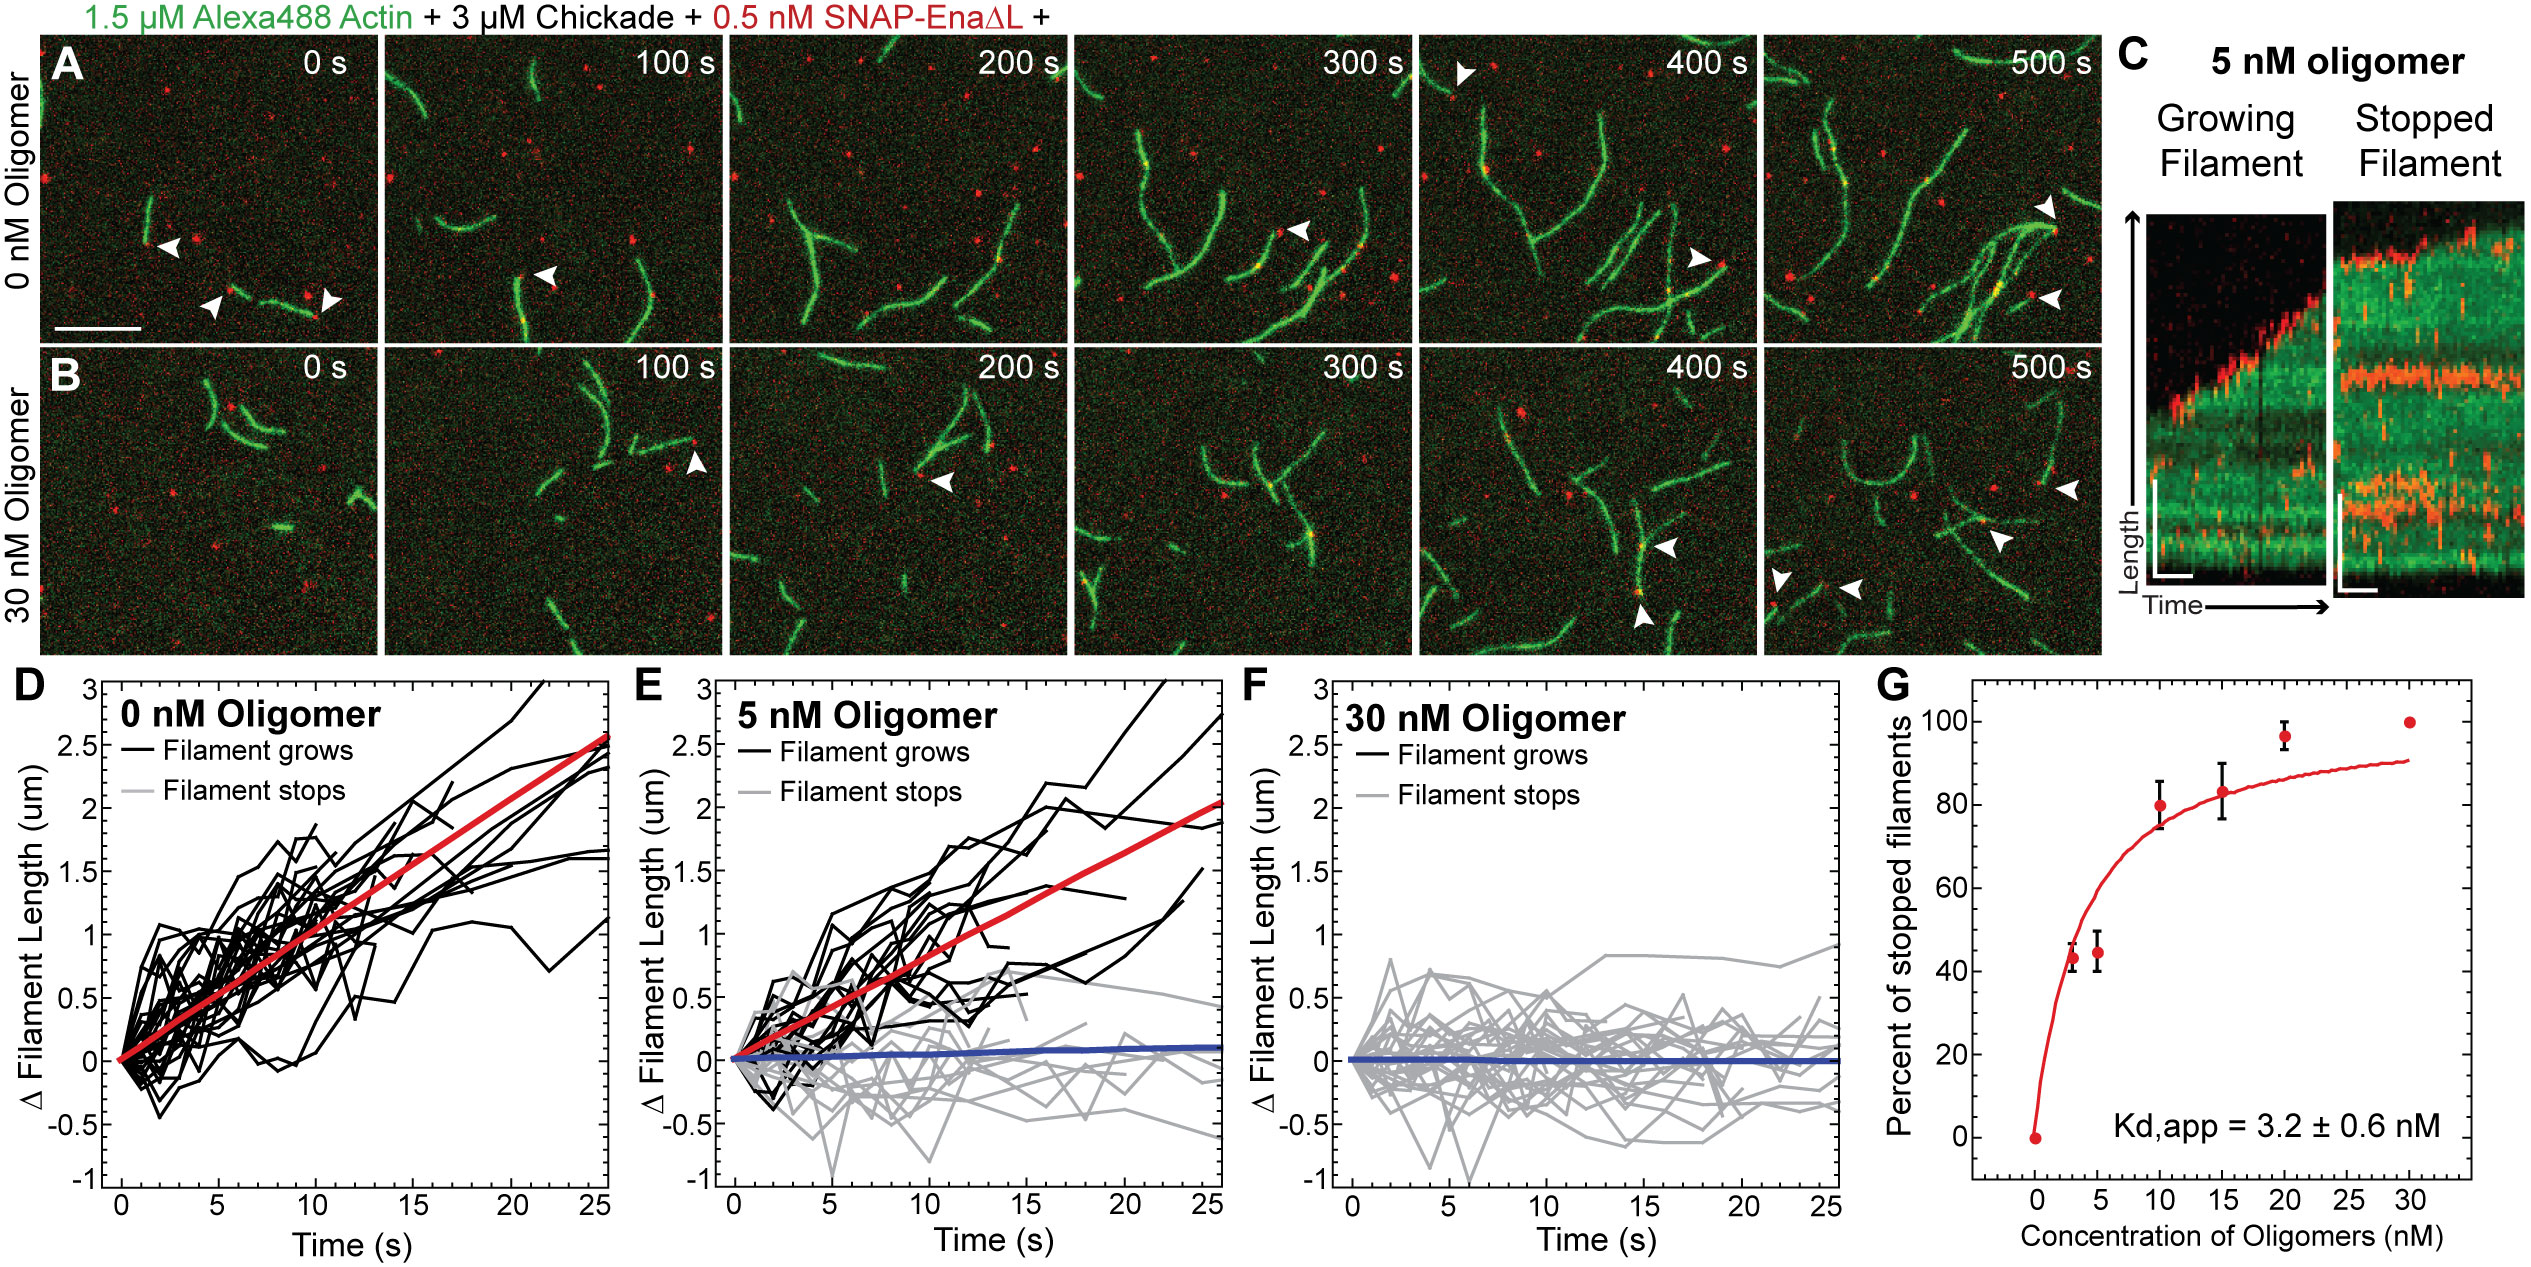
\includegraphics[width=\textwidth]{img/ch04/Oligomer_Ena_Figure.jpg}
\caption[Actin oligomers stop Ena mediated processive filament elongation.]{\textbf{Actin oligomers stop Ena mediated processive filament elongation.} Two color TIRFM timelapse of 1.5 $\mu$M Alexa-488 actin (green) and 0.5 nM SNAP-Ena$\Delta$L (red) in the presence of 3 $\mu$M Chickadee (fly profilin) and A) no actin oligomers or B) 30 nM actin oligomers. Arrows indicate Ena bound barbed ends. Scale bar, 10 $\mu$m. Kymographs of a G) growing Ena bound filament and a H) stopped Ena bound filament. Scale bar, 4 $\mu$m and 10 s. Filament elongation traces of Ena bound filaments with D) 0 nM Oligomers, E) 5 nM Oligomers, and F) 30 nM Oligomers. Red fit lines show average growth rates of Ena bound growing filaments and blue fit lines show average growth rates of Ena bound stopped filaments. C) Kd,app determined by TIRFM as percent of Ena bound stopped filaments over a range of actin oligomers. \textbf{Figure modified from \citep{kudryashova_actin_2018}}}
\label{fig:ena-oligomers}
\end{figure}

\subsection{VopL and VopF assemble endogenous actin}\label{vops}

As a part of understanding how VopF and VopL can assemble endogenous actin we observed that in the presence of profilin and G-actin, VopF and VopL bind to the pointed end of actin filaments to nucleate actin filaments. VopF and VopL will bind for a certain amount of time, or residence time, after nucleating the actin filament. We measured the residence time of VopL and VopF to understand its dynamics on pointed barbed ends. Since these proteins are nucleating actin filaments from G-actin, we made two different residence time calculations. The first calculation is from the observed timepoint where an actin filament and Vop protein are visualized with TIRFM. The second calculation takes into account how long before the filament is able to be visualized due to the resolution of the TIRFM. Overall we observe that both VopL and VopF bind to the pointed end of filaments for similar amounts of times. 

\begin{figure}
\centering
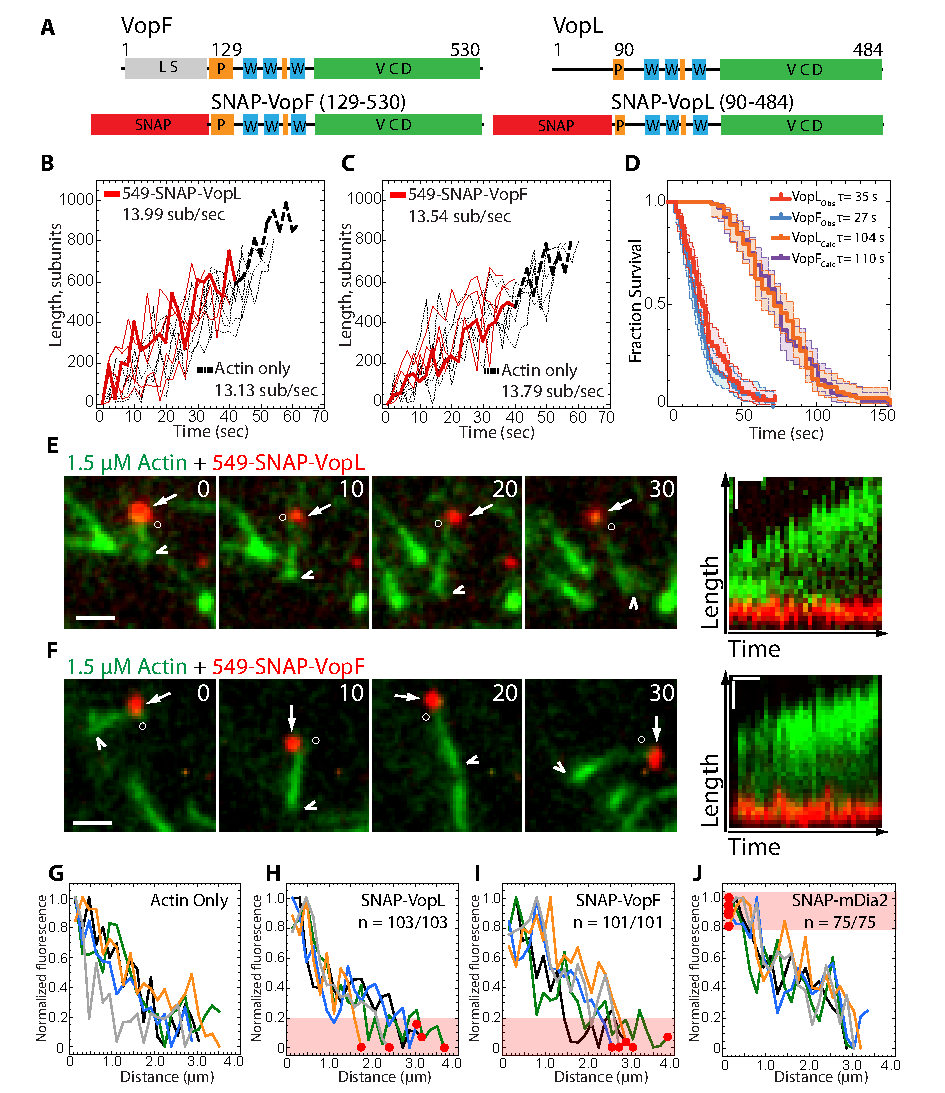
\includegraphics[width=\textwidth]{img/ch04/Thesis_Vop.pdf}
\caption[ VopL/F nucleate and then remain briefly associated with the pointed end of an actin filament.]{\textbf{ VopL/F nucleate and then remain briefly associated with the pointed end of an actin filament.} (A) Top, domain organization of VopL/F. Orange, proline-rich region (P); blue, WH2 domain (W); green, VCD dimerization domain. Bottom, VopL/F constructs used in this study with SNAP tag (red) for labeling. }
\label{fig:vop}
\end{figure}

% Continues caption on next page. Requires package ccaption.
\begin{figure}[!htb]
  \contcaption{(continued) (B–J) Slow acquisition (every 2 s, B–D) and rapid acquisition (every second, E–J) two-color TIRFM of the assembly of 1.5 $\mu$M Mg-ATP-actin (15\% Oregon green actin) with 0.2 nM 549(red)-SNAP-VopL/F. (B and C) Length of individual control (dashed black), 549-SNAP-VopL–associated (B, solid red), or 549-SNAP-VopF-associated (C, solid red) filaments over time ($n \geq 20$). (D) Kaplan–Meier curves representing the mean residence time of 549-SNAP-VopL/F on actin filaments observed (VopL\textsubscript{Obs}, VopF\textsubscript{Obs}) or assumed to have been associated because of nucleation (VopL\textsubscript{Calc}, VopF\textsubscript{Calc}). Error bars indicate 95\% CI; $n \geq 90$ events. (E and F, left) Merged timelapse micrographs (in seconds) of individual filaments. White arrowheads and open circles indicate bright and dim filament ends. White arrows indicate 549-SNAP-VopL/F. (E and F, right) Merged kymographs of filament length (y axis; bar, 1 $\mu$m) over time (x axis; bar, 10 s) of the corresponding filaments. Bars, 2 $\mu$m. (G–J) Linescans of the normalized fluorescence intensity of individual actin filaments measured from their bright to dim (bleached) ends. Red dots indicate position of 549-SNAP-VopL/F or 549-SNAP-mDia2 on the filament traces, and shaded red regions indicate where 100\% of VopL/F or mDia2 are bound to the filaments ($n \geq 75$). \textbf{TIRFM and linescans completed by Tom Burke. Figure modified from \citep{burke_bacterial_2017}.}}
\end{figure}

